%% ===================================================================
%% PART II
%% ===================================================================
\part{Circuit structure of non-embedded boxes}

%% -------------------------------------------------------------------
\section{The exact circuit-partition criterion}\label{sec:E1}

\begin{lemma}\label{lem:notunion}
A vector space $V$ over $\F_2$ is not the union of two proper subspaces.
\end{lemma}

\begin{proof}
If $\dim V=d$ and $A,B\subsetneq V$ are subspaces, then $|A\cup B|\le|A|+|B|-1\le2\cdot2^{d-1}-1<2^d$ because $0\in A\cap B$.
\end{proof}

(The statement is false for \emph{three} subspaces over $\F_2$, as the three lines of a plane show. This is why the criterion below is formulated with \emph{two} partitions.)

\begin{theorem}[Circuit-partition criterion; \gid{G10-E1}]\label{thm:E1}
For a code $C\le\F_2^n$ the following are equivalent.
\begin{enumerate}[label=(\roman*)]
\item The box $C$ is non-embedded.
\item There is a set $U\subseteq[n]$ with $|\Part_U(C)|\ge2$, i.e.\ $U$ has two distinct partitions into circuits.
\item Some word of $C$ has two distinct decompositions into disjoint circuits.
\end{enumerate}
Moreover, if $S\ne T$ are partitions of $U$ into circuits and $x\in C\setminus(\spn S\cup\spn T)$ (such $x$ exists), then $Z(S,x)$ and $Z(T,x)$ collide.
\end{theorem}

\begin{proof}
(ii)$\Leftrightarrow$(iii) is the identification of a word $\one_U$ with its support.

(ii)$\Rightarrow$(i). Let $S\ne T$ be partitions of $U$. By Lemma~\ref{lem:proper}, $\spn S$ and $\spn T$ are proper subspaces of $C_U\le C$, hence of $C$. By Lemma~\ref{lem:notunion} there is $x\in C\setminus(\spn S\cup\spn T)$. The cells $Z(S,x)$ and $Z(T,x)$ exist, have the same union $U$, agree (trivially) off $U$ because they have the same base point, and are different because $S\ne T$ (Lemma~\ref{lem:cellpair}). By Theorem~\ref{thm:centre} they collide.

(i)$\Rightarrow$(ii). Let $\{Z(S,x),Z(T,y)\}$ be a collision, so $U(S)=U(T)=:U$ and $x=y$ off $U$. If $S\ne T$ these are two distinct partitions of $U$. Suppose $S=T$. By Lemma~\ref{lem:cellpair} the cells are distinct, so $c:=x\oplus y\notin\spn S$; and $c\in C$ with $\supp c\subseteq U$ since $x=y$ off $U$. In particular $c\ne0$. By Lemma~\ref{lem:circuit-basic}(b) write $c=c_1\sqcup\dots\sqcup c_q$ as a disjoint union of circuits (all inside $U$). The word $\one_U\oplus c$ lies in $C$ (because $\one_U=\bigoplus S_j\in C$) and has support $U\setminus\supp c$; if this is nonempty write it as a disjoint union of circuits $d_1\sqcup\dots\sqcup d_s$. Then $S'=\{c_1,\dots,c_q,d_1,\dots,d_s\}$ is a partition of $U$ into circuits. If $S'=S$, every block of $S$ would lie either inside $\supp c$ or inside $U\setminus\supp c$, so $c$ would be a union of blocks of $S$, i.e.\ $c\in\spn S$, which is false. So $S'\ne S$ and $U$ has two distinct partitions.
\end{proof}

\src{\gid{G10-E1}, GEO-I v010, \texttt{MATHEMATICS.md} \S1.1 (\PROVED). The proof above uses only Lemmas~\ref{lem:proper} and~\ref{lem:notunion} and Theorem~\ref{thm:centre}. It was re-derived independently of the release text, and the equivalence (i)$\Leftrightarrow$(ii) was cross-checked by exhaustive computation on $4213$ small codes against a direct enumeration of cells and relative-interior intersections (Appendix~\ref{app:repro}); no discrepancy.}

\begin{remark}[Geometric content]\label{rem:E1geo}
Theorem~\ref{thm:E1} turns a metric--geometric property (overlap of relative interiors of parallelepipeds in $\R^n$) into a purely \emph{linear-algebraic} one (non-uniqueness of a decomposition into minimal supports). Two features are worth recording. First, the collision produced in (ii)$\Rightarrow$(i) uses a \emph{common} base point $x$ for both cells; collisions of this kind are the ones to which the rank-three construction of Section~\ref{sec:L5} applies. Second, in (i)$\Rightarrow$(ii) a collision with $S=T$ and distinct cosets forces a \emph{third} partition: this is the only place where one needs that every nonzero word is a union of circuits.
\end{remark}

\begin{proposition}[Cells through a centre]\label{prop:centre-count}
Let $U\subseteq[n]$ with $\one_U\in C$, let $C_U=\{w\in C:\supp w\subseteq U\}$ and let $z\in\F_2^{[n]\setminus U}$ be such that $X_z=\{x\in C: x|_{[n]\setminus U}=z\}$ is nonempty. The number of cells of positive dimension whose union is $U$ and whose base point agrees with $z$ off $U$ (that is, the cells whose relative interior contains the centre $\gamma(U,z)$) is
\[
N(U,z)=\sum_{S\in\Part_U(C)}\Bigl(\frac{|C_U|}{2^{|S|}}-[z=0]\Bigr).
\]
In particular, if $\one\in C$, then the number of cells whose centre is $(\tfrac12,\dots,\tfrac12)$ is $N=\sum_{P\in\Part}(2^{k-m_P}-1)$, with $m_P=|P|$ and $k=\dim C$, and the number of collisions with this centre is $\binom N2$.
\end{proposition}

\begin{proof}
$X_z$ is a coset of $C_U$ (the difference of two elements has support in $U$), so $|X_z|=|C_U|$. By Lemma~\ref{lem:cellpair} the cells over $(S,z)$ correspond to cosets of $\spn S\le C_U$ in $X_z$, excluding the coset $\spn S$ itself, which occurs inside $X_z$ exactly when $z=0$. The coset count is $|C_U|/2^{|S|}$ (Lemma~\ref{lem:span}). For $U=[n]$ the set $X_z$ is $C$ itself.
\end{proof}

\begin{corollary}[Collisions of a minimal box]\label{cor:collcount}
In a minimal non-embedded box every cell with $U=[n]$ has centre $\tfrac12\one$, every collision has this centre (Theorem~\ref{thm:F1}), and any two distinct cells with union $[n]$ collide. Hence the number of collisions is exactly $\binom N2$ with $N=\sum_{P\in\Part}(2^{k-m_P}-1)$.
\end{corollary}

\begin{proof}
A collision has a common union $U$ with two partitions, so $U=[n]$ by Theorem~\ref{thm:F1}; for $U=[n]$ the condition ``equal off $U$'' is empty, so any two distinct cells with union $[n]$ collide (Theorem~\ref{thm:centre}).
\end{proof}

\src{New here: this closed formula was not found in the release files read. It was verified by direct enumeration of cells for the $k=3,4,5$ classes (Appendix~\ref{app:repro}); e.g.\ $E_4$ has $N=3$ ($3$ collisions), the $k=4$, $p=6$ box has $N=13$ ($78$ collisions) and the $k=5$, $p=8$ box has $N=57$ ($1596$ collisions), in agreement with the direct enumeration of all collisions (Section~\ref{sec:E4}).}

%% -------------------------------------------------------------------
\section{Minimal non-embedded boxes and shortening}\label{sec:minimal}

\subsection{Shortening}

\begin{definition}[Shortening]\label{def:shortening}
For $i\in[n]$ the \emph{shortening} of $C$ at $i$ is the code $C_{(i)}=\{w|_{[n]\setminus\{i\}}:\ w\in C,\ w_i=0\}\le\F_2^{n-1}$. It is the kernel of the parity matrix with the $i$th column deleted. For $I\subseteq[n]$ write $C_{(I)}$ for the iterated shortening. The box $C_{(i)}$ is called a \emph{sub-box} of $C$.
\end{definition}

Deleting a column of $M$ corresponds geometrically to fixing the coordinate $i$ of every lattice vector at $0$: the lattice $\Lambda_{M'}$ of the deleted matrix is the intersection of $\Lambda_M$ with $\{\alpha_i=0\}$, and the box $[0,1]^{n-1}$ is the corresponding face of $[0,1]^n$.

\begin{lemma}[Circuits and cells of a shortening]\label{lem:shortcirc}
(a)~The circuits of $C_{(i)}$ are exactly the circuits of $C$ not containing $i$.
(b)~A circuit family of $C_{(i)}$ is a circuit family of $C$ avoiding $i$; the cells of $C_{(i)}$ are the cells $Z(S,x)$ of $C$ with $i\notin U(S)$ and $x_i=0$ (with coordinate $i$ deleted).
(c)~Two cells of $C_{(i)}$ collide if and only if the corresponding cells of $C$ collide, and the generator matrices of the pair differ only by an added zero column; so the witness ranks agree.
\end{lemma}

\begin{proof}
(a)~A word of $C_{(i)}$ is a word of $C$ vanishing at $i$. If $c$ is a circuit of $C$ with $i\notin c$ then every word of $C$ with support inside $c$ vanishes at $i$, so minimality in $C$ gives minimality in $C_{(i)}$. Conversely a circuit of $C_{(i)}$ is the support of a word of $C$ vanishing at $i$, and every word of $C$ with smaller support also vanishes at $i$, so it is a circuit of $C$ avoiding $i$. (b)~follows from (a) and the definition of cells, since $x\in C_{(i)}$ means $x\in C$, $x_i=0$. (c)~The condition ``same union and equal off the union'' reads the same in $\F_2^{n-1}$ and in $\F_2^n$ when $x_i=y_i=0$ and $i$ lies outside the common union.
\end{proof}

\begin{definition}[Minimal box]\label{def:minimal}
A box $C$ is \emph{minimal} (more fully: \emph{coordinatewise-minimal non-embedded}) if $C$ is non-embedded and $C_{(i)}$ is embedded for every $i\in[n]$.
\end{definition}

\begin{proposition}[Descent to a minimal sub-box]\label{prop:descent}
Every non-embedded box $C$ has a minimal sub-box $C_{(I)}$, $I\subseteq[n]$, and $\rmin(C)\le\rmin(C_{(I)})$.
\end{proposition}

\begin{proof}
If $C$ is non-embedded and not minimal, some $C_{(i)}$ is non-embedded and has length $n-1$. Repeat; the process stops because the length decreases at every step. By Lemma~\ref{lem:shortcirc}(c) every collision of $C_{(I)}$ lifts to a collision of $C$ with the same witness rank, so $\rmin(C)\le\rmin(C_{(I)})$.
\end{proof}

\src{\gid{G9-T5} (reduction to minimal boxes), GEO-I v009 \texttt{MATHEMATICS.md} \S2.4 (\PROVED+\CHECKED); the argument above is the general reduction without reference to nullity.}

\begin{corollary}[Nullity at least three]\label{cor:nullity}
If $C$ is non-embedded then $k=\dim C\ge3$.
\end{corollary}

\begin{proof}
By Theorem~\ref{thm:E1} there are partitions $S\ne T$ of some $U$. By Lemma~\ref{lem:proper}, $2\le|S|=\dim\spn S<\dim C_U\le k$, so $k\ge3$.
\end{proof}

\src{\gid{B-NULL$'$}, GEO-I v008 \texttt{MINIMAL\_RANK.md} (\PROVED): any collision forces nullity $\ge3$.}

\begin{figure}[ht]
\centering
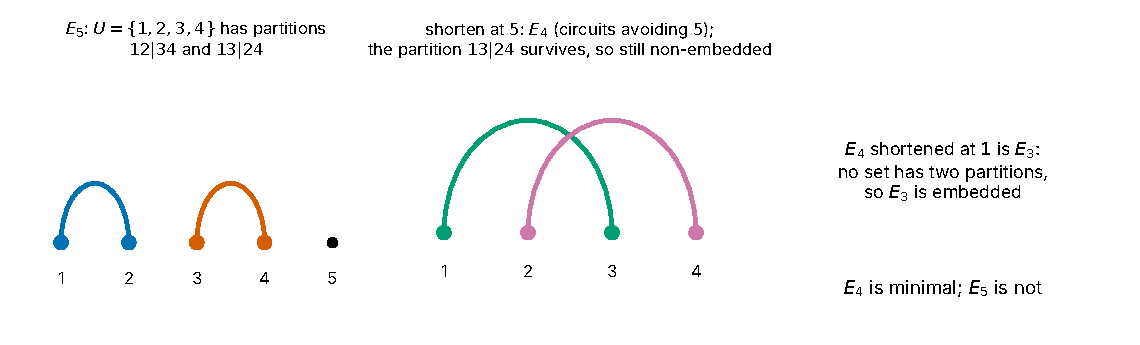
\includegraphics[width=0.95\textwidth]{figures/fig06_shortening.pdf}
\caption{Shortening a coordinate: deleting a parity column keeps exactly the circuits avoiding that coordinate. \figdesc{exact combinatorial data computed by \texttt{scripts/figs.py}; no higher-dimensional geometry is implied by the drawing.}}\label{fig:shortening}
\end{figure}

\subsection{Series classes and reduced boxes}\label{sec:series}

\begin{definition}[Series classes]\label{def:series}
Coordinates $i,j$ are \emph{series-equivalent} if $w_i=w_j$ for all $w\in C$. A coordinate is \emph{dead} if $w_i=0$ for all $w\in C$. The \emph{reduced length} $p(C)$ is the number of series classes of non-dead coordinates; the \emph{multiplicity} of a class is its size. The \emph{reduced code} $\bar C\le\F_2^{p}$ is obtained by keeping one coordinate from every class of non-dead coordinates (and deleting dead ones); $C$ is a \emph{blow-up} of $\bar C$ (plus dead coordinates).
\end{definition}

(In the generator-matrix picture of Section~\ref{sec:affine}, series-equivalent coordinates are the equal columns, and dead coordinates are the zero columns of a generator matrix; ``series'' and ``parallel'' are matroid names for the same relation, depending on whether one reads the code or its dual \cite{Oxley2011}. We use ``series''.)

\begin{proposition}[Blow-up invariance; \gid{B-SERIES}]\label{prop:series}
Let $C$ have no dead coordinates. The words of $C$ are constant on series classes, and replacing every class by a single coordinate gives an isomorphism $C\cong\bar C$ of codes. Under this isomorphism:
\begin{enumerate}[label=(\alph*)]
\item the circuits of $C$ are the preimages of the circuits of $\bar C$ (so every circuit is a union of classes);
\item cells correspond to cells, collisions to collisions; the generator matrices differ by duplicating columns, so witness ranks coincide and $\rmin(C)=\rmin(\bar C)$;
\item $C$ is non-embedded iff $\bar C$ is; and $C$ is minimal iff $\bar C$ is minimal.
\end{enumerate}
If $C$ has dead coordinates, the dead coordinates are in no circuit and in no cell; $C$ is non-embedded iff the code without the dead coordinates is, and then $C$ is not minimal.
\end{proposition}

\begin{proof}
Constancy on classes holds by definition and gives the isomorphism. Supports correspond to unions of classes and inclusion is preserved, so (a) follows; (b)~follows because union, equality off the union, and the cell data $(S,x)$ all transfer, and duplicating columns of a matrix does not change its row rank. For (c): non-embeddedness transfers by~(b). For minimality note that the circuits of $C_{(i)}$ are the circuits of $C$ avoiding $i$ (Lemma~\ref{lem:shortcirc}); these are the preimages of the circuits of $\bar C$ avoiding the class of $i$, i.e.\ the circuits of $\bar C_{(\bar\imath)}$; by Theorem~\ref{thm:E1} embeddedness of a shortening depends only on its circuits and the sets they form, so $C_{(i)}$ is embedded iff $\bar C_{(\bar\imath)}$ is. The statement on dead coordinates holds since a dead coordinate lies in no support, and $C_{(i)}$ for a dead $i$ is the code with $i$ deleted.
\end{proof}

\src{\gid{B-SERIES}, GEO-I v008 \texttt{MINIMAL\_RANK.md} (\PROVED+\CHECKED). Reproved above via Theorem~\ref{thm:E1}.}

\begin{remark}
A blow-up of a minimal box is minimal, although shortening a coordinate of a class of size $\ge2$ turns the other coordinates of the class into dead ones (zero columns of the generator matrix). This is consistent with Proposition~\ref{prop:series} because dead coordinates are irrelevant for embeddedness. Hence the classification of minimal boxes reduces to the classification of reduced minimal boxes plus multiplicities, and all rank statements for reduced boxes carry over to all lengths $n$ (Section~\ref{sec:classify}).
\end{remark}

%% -------------------------------------------------------------------
\section{The full-support theorem and zero-column exclusion}\label{sec:fullsupport}

\begin{theorem}[Full support; \gid{G10-F1}]\label{thm:F1}
Let $C$ be a minimal non-embedded box. If $U\subseteq[n]$ has two distinct partitions into circuits then $U=[n]$. Consequently $\one\in C$, the set $[n]$ has at least two partitions into circuits, and every coordinate lies in a circuit.
\end{theorem}

\begin{proof}
Let $S\ne T$ be partitions of $U$ and suppose $i\notin U$. All circuits of $S$ and $T$ avoid $i$, so by Lemma~\ref{lem:shortcirc}(a) they are circuits of $C_{(i)}$ and $S\ne T$ are two partitions of $U$ in $C_{(i)}$. By Theorem~\ref{thm:E1}, $C_{(i)}$ is non-embedded, contradicting minimality. By Theorem~\ref{thm:E1} some $U$ has two partitions; hence $U=[n]$ is the only such set. The word $\one=\one_{[n]}$ is then a sum of circuits, hence lies in $C$.
\end{proof}

\src{\gid{G10-F1}, GEO-I v010 \texttt{MATHEMATICS.md} \S1.2 (\PROVED); closes the earlier conjecture \gid{G8-C3} (status \textsc{corrected}: formerly open, now proved). This is an immediate consequence of the shortening lemma and Theorem~\ref{thm:E1}.}

\begin{proposition}[No singleton circuits; \gid{G9-Z}, \gid{G11-L5c}]\label{prop:nosingleton}
If $e_i\in C$ for some $i$ (that is, $\{i\}$ is a circuit; equivalently the $i$th parity column vanishes) and $C$ is non-embedded, then $C_{(i)}$ is non-embedded. Consequently a minimal non-embedded box has no circuit of size~$1$: every circuit has at least two coordinates, and there is no zero parity column.
\end{proposition}

\begin{proof}
Let $S\ne T$ be partitions of a set $U$ (Theorem~\ref{thm:E1}). If $i\notin U$ both are partitions in $C_{(i)}$ and we are done by Lemma~\ref{lem:shortcirc}. If $i\in U$, let $S_j\ni i$ be the block of $S$ containing $i$. Since $\{i\}$ is a circuit and circuits are not nested (Lemma~\ref{lem:circuit-basic}(c)), $S_j=\{i\}$; likewise $\{i\}\in T$. Then $S\setminus\{\{i\}\}$ and $T\setminus\{\{i\}\}$ are two different partitions of $U\setminus\{i\}$ (different because $S\ne T$; if one of them is empty then $S=\{\{i\}\}$, and $T$, being a partition of the same set containing $\{i\}$, would equal it). Both avoid $i$, so $C_{(i)}$ is non-embedded.
\end{proof}

\src{\gid{G9-Z}, GEO-I v009 \texttt{MATHEMATICS.md} \S1 (\PROVED+\CHECKED); \gid{G11-L5c}, GEO-I v011 \texttt{MATHEMATICS.md} \S1.1 (\PROVED). The two statements in the release files are proved by separate arguments; the single argument above gives both.}

\begin{corollary}[Properties of a minimal box]\label{cor:minprops}
A minimal non-embedded box $C$ of nullity $k$ satisfies: (P1)~$\one\in C$ and $|\Part|\ge2$; (P2)~no coordinate is dead; every circuit has at least two coordinates; (P3)~$k\ge3$ and $\one$ is not a circuit; (P4)~every partition of $\one$ has $m_P\ge2$ blocks of size $\ge2$ each.
\end{corollary}

\begin{proof}
(P1)~Theorem~\ref{thm:F1}. (P2)~$\one\in C$ has full support, and Proposition~\ref{prop:nosingleton}. (P3)~Corollary~\ref{cor:nullity}; if $\one$ were a circuit then every circuit equals $\one$ and $\Part$ has a single element. (P4)~is (P2) together with (P3).
\end{proof}

%% -------------------------------------------------------------------
\section{Affine-geometric reduction}\label{sec:affine}

\subsection{Generator matrices and point sets}

Let $C\le\F_2^n$ be a code of dimension $k$ without dead coordinates. Choose a basis $b_1,\dots,b_k$ of $C$ and let $G$ be the $k\times n$ matrix with rows $b_s$. Its columns $g_1,\dots,g_n\in\F_2^k\setminus\{0\}$ satisfy
\[
w_f:=\bigl(f\cdot g_i\bigr)_{i\in[n]}\in C,\qquad C=\{w_f:\ f\in\F_2^k\},\qquad f\mapsto w_f\ \text{bijective}.
\]
Thus a code of dimension $k$ without dead coordinates is a \emph{multiset} of nonzero points of $F_2^k$ spanning $\F_2^k$ (the column multiset), up to the action of $\GL(k,2)$ (change of basis of $C$) and permutation of coordinates. Series classes are the sets of coordinates with equal columns; the reduced code corresponds to the set $X=\{g_i\}$ of \emph{distinct} columns, $|X|=p$, spanning $\F_2^k$.

\begin{lemma}\label{lem:equivalence}
Two reduced codes $\bar C,\bar C'$ with point sets $X,X'\subseteq\F_2^k\setminus\{0\}$ (spanning) are equal up to a permutation of coordinates if and only if $X'=\sigma X$ for some $\sigma\in\GL(k,2)$.
\end{lemma}

\begin{proof}
If $\pi\bar C=\bar C'$ for a coordinate permutation $\pi$, then $G'\Pi=AG$ for an invertible $A$ (two generator matrices of the same code differ by a change of basis), so the column of $G'$ at position $\pi(i)$ is $Ag_i$: $X'=AX$. Conversely if $X'=\sigma X$ then $G'$, whose columns are $\sigma g_i$ in some order, generates $\{f\cdot\sigma g_i\}=\{(\sigma^{\top}f)\cdot g_i\}$, the same code up to the coordinate order.
\end{proof}

\begin{figure}[ht]
\centering
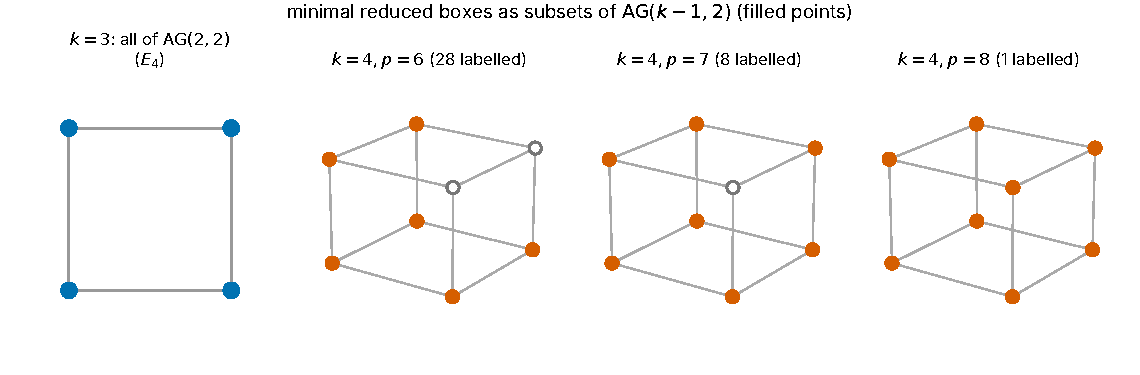
\includegraphics[width=0.95\textwidth]{figures/fig07_affine_reduction.pdf}
\caption{Affine reduction: the reduced coordinate set as a point set in an affine space. \figdesc{exact combinatorial data computed by \texttt{scripts/figs.py}; no higher-dimensional geometry is implied by the drawing.}}\label{fig:affred}
\end{figure}

\subsection{The affine hyperplane}

Since $\one\in C$ for minimal boxes (Theorem~\ref{thm:F1}) there is a unique $f_0\in\F_2^k$ with $w_{f_0}=\one$, i.e.\ $f_0\cdot g_i=1$ for all $i$. The set $H=\{x\in\F_2^k: f_0\cdot x=1\}$ is an affine hyperplane, in bijection with $\F_2^{k-1}$ after choosing coordinates in which $f_0=e_k^*$, and its affine structure is that of the affine space $\AG(k-1,2)$ (the points of $H$ are the vectors with last coordinate $1$). The subgroup of $\GL(k,2)$ preserving $H$ (equivalently fixing $f_0$) acts on $H$ as the full affine group $\AGL(k-1,2)$.

\begin{theorem}[Affine reduction; \gid{G10-A1}]\label{thm:affine}
Let $C$ be a minimal non-embedded box of nullity $k$ and $X\subseteq\F_2^k$ its reduced point set, $p=|X|$. Then:
\begin{enumerate}[label=(\alph*)]
\item $X\subseteq H\cong\AG(k-1,2)$ and $X$ spans $\F_2^k$ (equivalently, $X$ is not contained in any proper affine subspace of $H$);
\item $p\ge k+1$; and $p=k+1$ holds if and only if $C=E_p$ (and then $p=4$, $k=3$);
\item two minimal boxes have isomorphic reduced codes iff their reduced point sets lie in the same $\AGL(k-1,2)$-orbit of subsets of $H$.
\end{enumerate}
Conversely, for every spanning subset $X\subseteq H$ the code $C(X)=\{(f\cdot x)_{x\in X}\}$ has dimension $k$ and contains $\one$; whether it is non-embedded, and whether it is minimal, depends on $X$ only through its $\AGL(k-1,2)$-orbit.
\end{theorem}

\begin{proof}
(a)~$\one\in C$ gives $X\subseteq H$; $X$ spans because the generator matrix has rank $k$; and ``spans $\F_2^k$'' means that $X$ is not contained in a proper linear subspace; since $X\subset H$ and $0\notin H$, this means $X$ is not contained in a proper affine subspace of $H$.

(b)~$p=k$ would make $X$ a basis, so $C=\F_2^p$ with all singletons as circuits, contradicting Proposition~\ref{prop:nosingleton}. For $p=k+1$ the relations among the columns form a $1$-dimensional space $\langle a\rangle=C^\perp$, hence $C=a^\perp$. If $a_i=0$ then $e_i\in C$, a singleton circuit; so $a=\one$, $C=\one^\perp=E_p$. (The circuits of $E_p$ are the weight-two words, and $E_p$ is minimal only for $p=4$, Proposition~\ref{prop:Emin}.)

(c)~Lemma~\ref{lem:equivalence} gives equivalence under $\GL(k,2)$. If $\sigma X=X'$ and both sets lie in $H$, then $\sigma$ maps $X$ into $H$; because $X$ spans, $f_0\circ\sigma^{-1}$ takes the value $1$ on $X'$, which spans, and is a functional equal to $1$ on a spanning subset of $H$, so $f_0\circ\sigma^{-1}=f_0$ (a functional is determined by its values on a spanning set). So $\sigma$ lies in the stabiliser of $f_0$, which acts on $H$ as $\AGL(k-1,2)$.

The final statement is Lemma~\ref{lem:equivalence} together with the fact that isomorphic codes have the same circuits and hence the same embeddedness and minimality (Theorem~\ref{thm:E1}).
\end{proof}

\src{\gid{G10-A1}, GEO-I v010 \texttt{MATHEMATICS.md} \S1.3 (\PROVED). The statements on $p\ge k+1$ and on $E_p$ are made explicit here.}

\begin{proposition}[The even-weight codes]\label{prop:Emin}
For $p\ge3$ let $E_p=\{w\in\F_2^p:\wt(w)\text{ even}\}$. Its circuits are the $\binom p2$ words of weight two. $E_3$ is embedded, $E_p$ is non-embedded for $p\ge4$, $E_4$ is minimal, and $E_p$ is not minimal for $p\ge5$.
\end{proposition}

\begin{proof}
Every even word of weight $\ge4$ contains a weight-two word, so the circuits are the pairs. A family of disjoint pairs is a partial matching; $E_3$ has no two disjoint pairs, so the families are single pairs and every set has at most one partition: embedded. For $p\ge4$ the set $\{1,2,3,4\}$ has the partitions $\{12,34\}$ and $\{13,24\}$: non-embedded. Shortening $E_p$ at a coordinate gives $E_{p-1}$ (the words vanishing at $i$ are the even words on the other coordinates), so $E_4$ has the embedded shortening $E_3$, while for $p\ge5$ the shortening $E_{p-1}$ with $p-1\ge4$ is non-embedded.
\end{proof}

\subsection{Consequences}

Theorem~\ref{thm:affine} reduces the study of minimal boxes to the study of subsets of the finite affine spaces $\AG(k-1,2)$ up to affine equivalence. It also fixes the extreme case: the full affine space $X=\AG(k-1,2)$, which gives the first-order Reed--Muller code $\mathrm{RM}(1,k-1)$ of length $2^{k-1}$ (Proposition~\ref{prop:RM}). All the arithmetic below is done with $k$ (the dimension of the ambient space $\F_2^k$), $p$ (the number of points) and the partition data of $X$.

%% -------------------------------------------------------------------
\section{Collision rank and local rank-three extraction}\label{sec:L5}

\begin{lemma}[Lower bound; \gid{B-LOW}]\label{lem:LOW}
Every collision has witness rank at least $3$. Consequently $\rmin(C)\ge3$ for every non-embedded box.
\end{lemma}

\begin{proof}
Let $\{Z(S,x),Z(T,y)\}$ be a collision, $r=|S|,t=|T|$, with generators $g_j$ and $h_l$. By Lemma~\ref{lem:rankspan} the witness rank is at least $\max(r,t)$, so we may assume $r,t\le2$.

\emph{Case $r=1$.} Then $U=S_1$ is a circuit, so every circuit inside $U$ equals $U$ and $T=\{U\}=S$. As $x=y$ off $U$, the word $c=x\oplus y$ has support in $U$, so $c\in\{0,U\}=\spn S$ (Lemma~\ref{lem:circuit-basic}(c)), and $Z(S,x)=Z(S,y)$ by Lemma~\ref{lem:cellpair}, a contradiction. The case $t=1$ is symmetric. So $r=t=2$.

\emph{Case $r=t=2$.} Suppose the witness rank equals $2$. Then the rows of $B$ lie in the row space of $A$: $h_l=\lambda_{l1}g_1+\lambda_{l2}g_2$ with real $\lambda$. Since $g_j$ has entries $\pm1$ exactly on $S_j$ and $h_l$ has entries in $\{0,\pm1\}$, $|\lambda_{lj}|\in\{0,1\}$. If both were nonzero then $T_l=S_1\cup S_2=U$ and the other member of $T$ could not be disjoint from it; so each $T_l$ equals $S_1$ or $S_2$, and $T=S$. Then $h_l=\pm g_l$ means $1-2y_i=\varepsilon_l(1-2x_i)$ on $S_l$, i.e.\ $y|_{S_l}=x|_{S_l}$ or $y|_{S_l}=\bar x|_{S_l}$ for each $l$; hence $c=x\oplus y$ is constant on every block, so $c\in\spn S$ (it vanishes off $U$ because $x=y$ there), and the cells coincide: a contradiction. So the rank is at least $3$.
\end{proof}

\src{\gid{B-LOW} (also \gid{G8-T3a}), GEO-I v008 \texttt{MINIMAL\_RANK.md} (\PROVED).}

\begin{theorem}[Local rank-three extraction; \gid{G10-L5}, \gid{B-COMMON}]\label{thm:L5}
Let $a\in C$ be a word with two distinct decompositions into two disjoint circuits, $a=b_1\sqcup b_2=c_1\sqcup c_2$ with $\{b_1,b_2\}\ne\{c_1,c_2\}$. Put $S=\{b_1,b_2\}$, $T=\{c_1,c_2\}$ and choose any $x\in C\setminus(\spn S\cup\spn T)$. Then $Z(S,x)$ and $Z(T,x)$ collide, and their four generators satisfy
\[
g_1+g_2=h_1+h_2=\bigl((1-2x_i)\one_{i\in\supp a}\bigr)_{i\in[n]},
\]
so the witness rank is exactly $3$. In particular $\rmin(C)=3$ for any code that contains such a word.
\end{theorem}

\begin{proof}
Theorem~\ref{thm:E1} gives the collision. On $U=\supp a$ the generators of the two cells are the restrictions of the same vector $s=(1-2x_i)_i$ to the blocks: $g_j=s|_{b_j}$, $h_l=s|_{c_l}$. Hence $g_1+g_2=s|_U=h_1+h_2$, a nontrivial linear relation among four vectors; their span has dimension at most $3$. Lemma~\ref{lem:LOW} gives at least $3$.
\end{proof}

\src{\gid{G10-L5} (= \gid{G10-T5}) and \gid{B-COMMON}, GEO-I v010 \texttt{MATHEMATICS.md} \S1.5 and v008 \texttt{MINIMAL\_RANK.md} (\PROVED).}

\begin{definition}[Condition W2]\label{def:W2}
A box satisfies \emph{W2} if $\one\in C$ and the set $\Part^{(2)}$ of partitions of $\one$ into exactly two circuits has at least two elements; $n_2=|\Part^{(2)}|$.
\end{definition}

\begin{theorem}[Conditional universality; \gid{G10-C1$'$}]\label{thm:C1p}
If every minimal non-embedded box satisfies W2, then $\rmin(C)=3$ for \emph{every} non-embedded box $C$.
\end{theorem}

\begin{proof}
By Proposition~\ref{prop:descent} there is a minimal sub-box $C_{(I)}$ with $\rmin(C)\le\rmin(C_{(I)})$. By W2 the word $\one\in C_{(I)}$ has two distinct two-circuit decompositions, so Theorem~\ref{thm:L5} gives $\rmin(C_{(I)})=3$. Hence $\rmin(C)\le3$, and Lemma~\ref{lem:LOW} gives $\rmin(C)\ge3$.
\end{proof}

\src{\gid{G10-C1$'$}, GEO-I v010 \texttt{MATHEMATICS.md} \S1.5 (\PROVED). The hypothesis W2 for \emph{all} minimal boxes is the content of Theorem~\ref{thm:W2} (Part~III), proved unconditionally in this paper.}

Theorem~\ref{thm:C1p} thus reduces the universal rank statement to a purely combinatorial one: \emph{every minimal non-embedded box has two distinct partitions of the all-ones word into two circuits}. Part~III proves this.

\begin{figure}[ht]
\centering
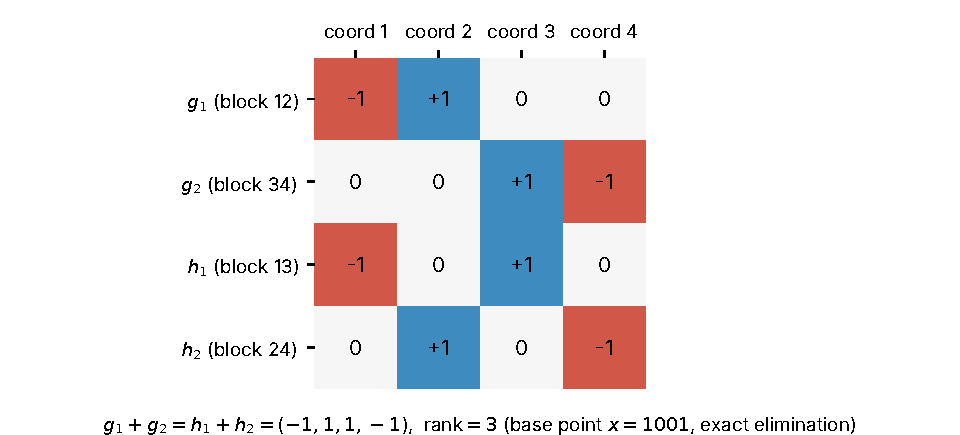
\includegraphics[width=0.95\textwidth]{figures/fig05_rank3_collision.pdf}
\caption{A rank-three collision in $E_4$ with common base point $x=1001$. The four generators of the cells $Z(\{12,34\},x)$ and $Z(\{13,24\},x)$ as a $4\times4$ matrix, and the relation $g_1+g_2=h_1+h_2=(-1,1,1,-1)$. \figdesc{exact integer data; rank computed by exact elimination, \texttt{scripts/figs.py}.}}\label{fig:rank3}
\end{figure}

\begin{figure}[ht]
\centering
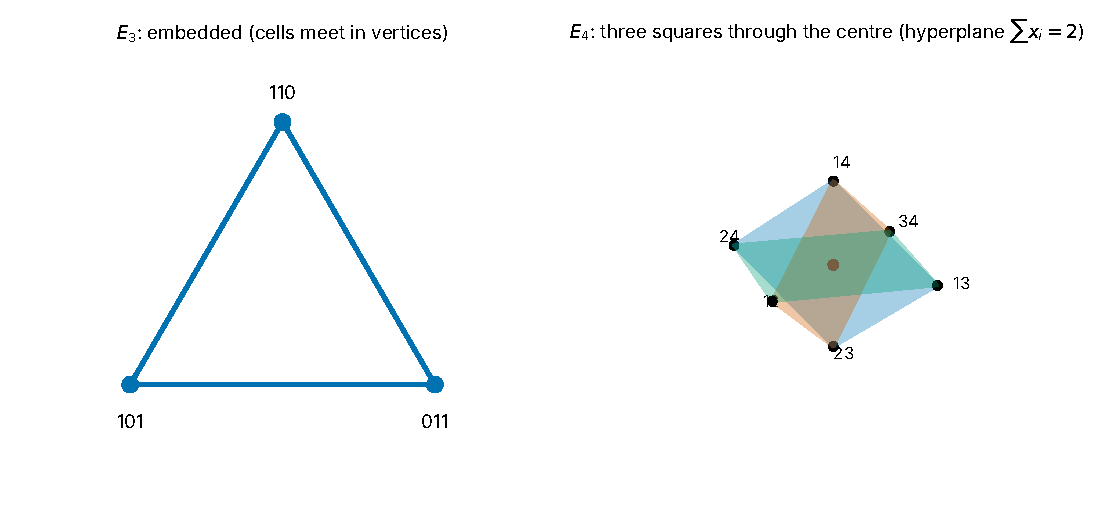
\includegraphics[width=0.95\textwidth]{figures/fig04_embedded_vs_nonembedded.pdf}
\caption{Embedded versus non-embedded. Left: $E_3$ (a triangle; cells meet in vertices). Right: the octahedron of the six weight-two words of $E_4$ in the hyperplane $\sum x_i=2$ with the three equatorial squares, which share diagonals and all contain the centre. \figdesc{an exact subcomplex of the $4$-dimensional cell structure; the vertex $1111$ and the cells through it are omitted. Not a picture of the full cell complex.}}\label{fig:octa}
\end{figure}
